\section{Background}
\label{sec:background}

\subsection{Brief introduction to SystemJ syntax, semantics and model of
  computation}
\label{sec:brief-intr-syst}

\begin{table}[tb]
\centering
\caption{SystemJ kernel statements and their meaning}
\begin{minipage}{8cm}
  \begin{scriptsize}
   \begin{tabular}{|c|p{80pt}|}
     \hline                                                                                     
     \textbf{Kernel Statements} & \textbf{Meaning}\\                                            
     \hline                                                                                     
     \hline                                                                                     
     [\textbf{\texttt{input}}] [\textbf{\texttt{output}}]
     [\textbf{\texttt{type}}] \textbf{\texttt{signal}} S & declare signal S\\                                      
     \hline                                                                                     
     \textbf{\texttt{emit}} S [(value)] & broadcast signal S\\                                                    
     \hline                                                                                     
     \textbf{\texttt{present}} (S) \{p\} else \{q\}& do p if S is present, else do q\\                            
     \hline                                                                                     
     \textbf{\texttt{abort}} (S) \{p\} & preempt program p if S is present\\                                      
     \hline                                                                                     
     \textbf{\texttt{suspend}} (S)\{p\} & suspend p if S is present\\                                             
     \hline                                                                                     
     \textbf{\texttt{trap}} (T)\{p\ldots \textbf{\texttt{exit}} T\ldots\} & preempt p if exit is executed\\                         
     \hline                                                                                     
     p\textbf{\texttt{$||$}}q & run p and q in lock-step\\                                                        
     \hline                                                                                     
     p$><$q & run p and q asynchronously\\                                                      
     \hline                                                                                     
     \textbf{\texttt{send}} C([value]) & send a value through C, blocking
     send\\                                                 
     \hline                                                                                     
     \textbf{\texttt{receive}} C() & receive a value through C, blocking
     receive\\
     \hline                                                                                     
     \textbf{\texttt{pause}} & finish a tick and communicate
     with environment\\
     \hline                                                                                     
   \end{tabular}
  \end{scriptsize}
   % \footnotetext[1]{\scriptsize Uppercase}
 \end{minipage}
 \label{tab:1}
\end{table}

Table~\ref{tab:1} presents the SystemJ kernel statements used to program
the control flow. The data flow is programmed in the safe subset of
Java~\cite{scj2013} amenable to formal verification and timing analysis,
while avoiding all the pitfalls of programming in `C' style languages. A
number of derived statements also exist (e.g., \texttt{sustain},
\texttt{await}, etc) that make programming reactive systems easier. The
\textit{Model of Computation} (MoC) of a simple SystemJ program is shown
in Figure~\ref{fig:2}.

SystemJ consists of entities called \textit{Clock Domains} (CD)s, each
running at their individual pace, interacting with the environment via
signals and with each other via channels and CSP~\cite{choa85} style
rendezvous. Each CD has its own notion of logical time. CDs adhere to
the \textit{perfect synchrony} hypothesis, i.e., all statements execute
instantaneously in zero time. Only the \texttt{pause} statement consumes
time, just like in Esterel~\cite{gber931}. Consider the SystemJ program
in Figure~\ref{fig:2a}, it is waiting for an input signal producing
logical ticks (see Figure~\ref{fig:2c}). Once \texttt{A} is received at
tick 1 or 4, output \texttt{O} is emitted to the environment
instantaneously.

\subsection{Mapping logical time to physical time}
\label{sec:mapping-logical-time}

\begin{figure}[t!]
\centering
\begin{SubFloat}{\label{fig:2a}Simple SystemJ program}%...verbatim subfigure
\begin{minipage}[b]{1\linewidth}% a minipage to control the width...
		\begin{lstlisting}[style=sysj,morekeywords={abort,await,emit,present,trap,pause,exit,delay,suspend}]
{
int counter = 0;
while(true){
 abort(immediate A){
  while(true) pause; 
 } // abort end
  emit O;
  if(counter != 0) {/* java computation leading to WCRT */}
  ++counter;
 } // loop end
} // SystemJ CD end
\end{lstlisting}%
\end{minipage}%
\end{SubFloat}
%\hspace{1.5cm}%
% \begin{SubFloat}[Black box]{\label{fig:2b}Logical time in SystemJ}%
% 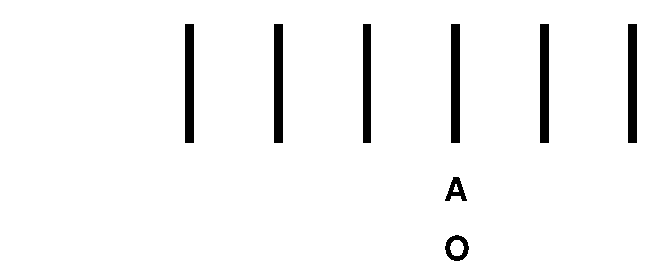
\includegraphics[scale=0.4]{moc}
% \end{SubFloat}%
% \vspace{-10pt}

\begin{SubFloat}{\label{fig:2c}Mapping to physical time}%
% \includegraphics[scale=0.4]{phy.pdf_t}
\scalebox{0.68}{\input{phy.pdf_t}}
\end{SubFloat}%
\caption{Simple SystemJ example and corresponding MoC}
\label{fig:2}
\end{figure}

The perfect synchrony hypothesis is ideal for programming the
synchronous sub-set of SystemJ. Unfortunately, execution of every
statement in the logical zero time requires $\delta$ physical time. Time
for a logical tick can thus be summarized as $\Delta = \mathcal{F}
(\delta)$, where $\mathcal{F}$ is the schedule. We call $\Delta$ the
reaction time. Depending upon the amount of computation required and
schedule, $\Delta$ can vary. In order to satisfy the implicit
restriction imposed by the synchrony hypothesis -- no input event
\textit{from the environment} can be missed -- one needs to calculate
the \textit{Worst Case Reaction Time} (WCRT) and the resultant WCRT
needs to be smaller than the time between any two consecutive events on
any input, else the synchrony hypothesis is violated. Techniques for
calculating the WCRT of synchronous programs~\cite{boldt07} exist and
this analysis is not the focus of this paper. The opposite of the WCRT,
the shortest time for a reaction, is called the \textit{Best Case
  Reaction Time} (BCRT). Formally, let $\{\Delta_1, \Delta_2,\ldots,
\Delta_N\}$, be the set of all possible reaction times for some
CD. Then, $\exists i \in N, s.t., WCRT= max (\Delta_i)$ and $\exists j
\in N, s.t., BCRT = min (\Delta_j)$.


We denote the WCRT and BCRT in Figure~\ref{fig:2c} using \texttt{W} and
\texttt{B}, respectively. Figure~\ref{fig:2c} shows a continuously
running physical clock (analogous to a clock in digital hardware), the
numerical annotations on the rising edge of the clock mark the logical
ticks from Figure~\ref{fig:2c}. The subscripts \texttt{s} and \texttt{e}
for the numbers show the start and end of the logical ticks,
respectively. The end of a logical tick and the start of the next
logical tick happen together. Figure~\ref{fig:2c} shows the mapping of
the logical time to the physical time. For example, the logical tick
\texttt{1} starts at the first rising edge and completes at the second
rising edge of the physical clock, whereas logical tick \texttt{4}
starts at the $4^{th}$ rising edge, but finishes at the $6^{th}$ rising
edge of the physical clock. This difference can be accounted for by the
Java computations required when signal \texttt{A} is input by the
environment (see Figure~\ref{fig:2a}). This elasticity is inherent (and
elegant) to both Esterel and SystemJ.

% We now present a lemma with proof sketch (due to lack of space) that we
% require for the rest of the paper and is special to SystemJ, being a
% GALS language.

% \begin{lemma}
%   WCRT and BCRT analysis are invariant to values of conditional
%   expressions.
% \end{lemma}

% \begin{proof}
%   The physical time ($\delta$) taken by a conditional expression is at
%   best affected by the type rather than the value of the
%   conditional. Example, comparing the value of 2 floats might take
%   longer than comparing the value of 2 integer types on some given
%   platform. But, the time taken by the comparison instruction is
%   invariant to the value itself.
% \end{proof}

% \begin{lemma}
%   WCRT and BCRT analysis are invariant to channel communication.
% \end{lemma}
% \begin{proof}
%   LATER ....
% \end{proof}


%%% Local Variables: 
%%% mode: latex
%%% TeX-master: "paper"
%%% End: 
